\sekshun{Rectangle Integration}
\label{Rectangle_Integration}

\begin{seamlessnote}
  Now that we have our requirements documented, it is time to enter into the repetitive \seamless
  TDD cycles necessary to actually document, test, and develop our code. First, some suggestions:
  \begin{itemize}
    \item there should be example programs for every package feature
    \item in explaining a feature, try to address everyone in your audience
      (e.g. the package developers as well as the black box users)
    \item explain the syntax of the feature and any implementation details
    \item explain the impact of the feature and how it is used when piecing together
      an application
    \item italicize a term when you are defining it and be sure to add it to the 
      index (more on index creation below)  
  \end{itemize}

  In our toy example, we are developing a few numerical integration methods, and we begin with a description
  of the rectangle method. What follows is a just normal \latex prose including a figure generated in Mathematica
  to illustrate the concept. It is a good idea to include any external scripts, programs, or spreadsheets used to
  generate figures for your documentation, and the Mathematica notebook for generating Figure~\ref{fig:rectangle}
  is included with the tutorial in the \path{./tutorial/Mathematica} directory.
\end{seamlessnote}

The \textit{rectangle integration method}\index{rectangle integration method}\index{integration method!rectangle}
computes an approximation to a 
definite integral by finding the area of a collection of rectangles whose heights are determined 
by the values of the function.  Specifically, the interval $[a,b]$ over which the function is to 
be integrated is divided into $N$ equal subintervals of length $h = (b-a)/N$. The rectangles are 
drawn with one base along the $x$-axis. Depending on whether the method is left, right, or midpoint,
the left corner, right corner, or midpoint, respectively, of the side opposite the base lies on the 
graph of the function. The approximation to the integral is 
then calculated by adding up the areas (base multiplied by height) of the $N$ rectangles, 
giving the formula:
\begin{equation}
  \int_a^b f(x) dx \approx h \sum_{n=0}^{N-1} f(x_n) \label{eq:rectangle}
\end{equation}
where
\begin{equation}
  h=(b-a)/N  \label{eq:subinterval-width}
\end{equation}

\begin{seamlessnote}
  Notice that the term ``rectangle integration method'' above is italicized at its first use. If you look 
  in the index at the end of the tutorial, you will see two different entries for the term. 
  One is a plain entry for ``rectangle
  integration method,'' and the other is a subentry for ``rectangle'' under the ``integration method'' entry. 
  The index entries are created by inserting \verb|\index| commands in the \latex source and running
  the \verb|makeindex| command (included for you in the \verb|Makefile|). The plain entry
  is inserted by simply entering \verb!\index{rectangle integration method}! after the first
  occurrence of the term. The subentry is inserted by using a \verb|!| to annotate the subentry after the main entry
  (\eg \verb|\index{integration method!rectangle}|).  Some things to consider with respect to
  index term creation:
  \begin{itemize}
    \item enter as many terms as possible into the index; it is better to err on the side of too 
      many entries; you can cull excessive entries later
    \item double-billing is encouraged (\eg \verb|\index{formal arguments}|, 
      \\ \verb|\index{arguments!formal}|)
    \item an acceptable exception to double-billing is when the entries are visually close 
      \\ (\eg \verb|\index{operator precedence}|, \verb|\index{operators!precedence}|), and
      in this case, the second form is preferred
    \item global topics can appear at the top level; otherwise, they are qualified by
      the chapter name (or general topic)
  \end{itemize}
\end{seamlessnote}

The formula for $x_n$ for the left, right, and midpoint methods are given in Table \ref{tab:xn-rectangle}.
As $N$ gets larger, the rectangle method becomes more accurate. This is illustrated in the series of plots
in Figure \ref{fig:rectangle}.

\begin{table}[htbp]
  \centering
  \caption{Formula for $x_n$ in Equation \ref{eq:rectangle} of 
  rectangle numerical integration methods.} 
  \label{tab:xn-rectangle}
  \begin{tabular}{cc}
    \textbf{Method} & \textbf{$x_n$} \\ \toprule
    left & $a+nh$ \\ \midrule
    right & $a+(n+1)h$ \\ \midrule
    midpoint & $a+\left(n + \frac{1}{2}\right)h$ \\ \bottomrule
  \end{tabular}
\end{table}

\begin{figure}
  \centering
  \subcaptionbox{$N=4$}{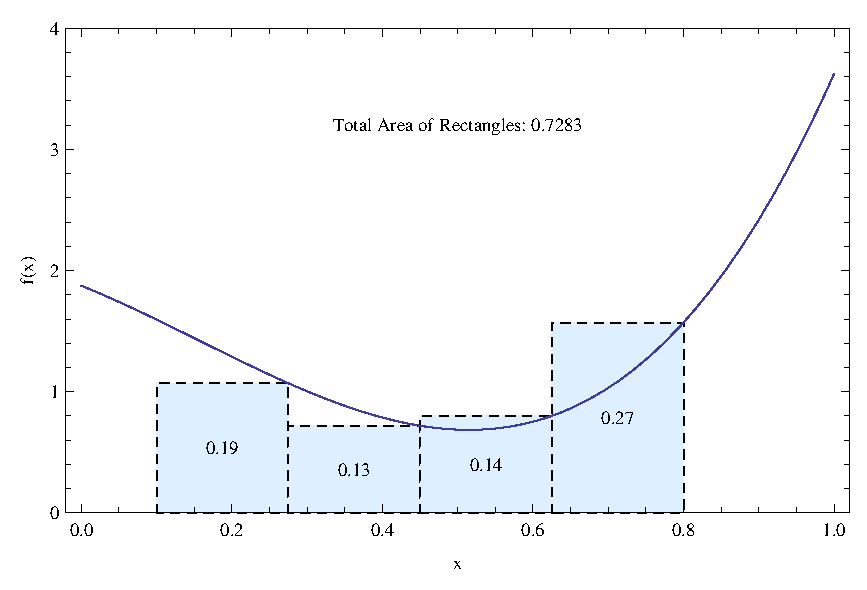
\includegraphics[scale=.6]{fig/rightrectangle-4.eps}}
  \subcaptionbox{$N=6$}{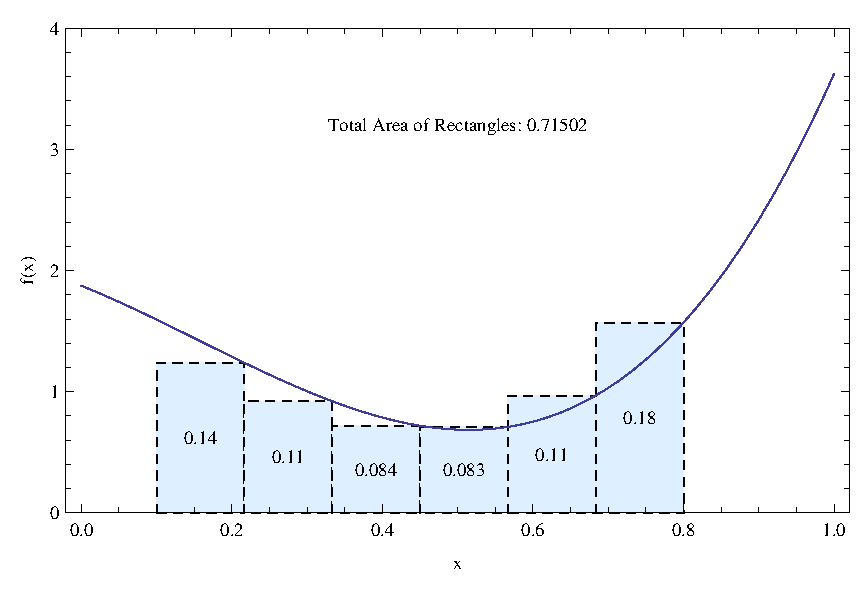
\includegraphics[scale=.6]{fig/rightrectangle-6.eps}}
  \subcaptionbox{$N=10$}{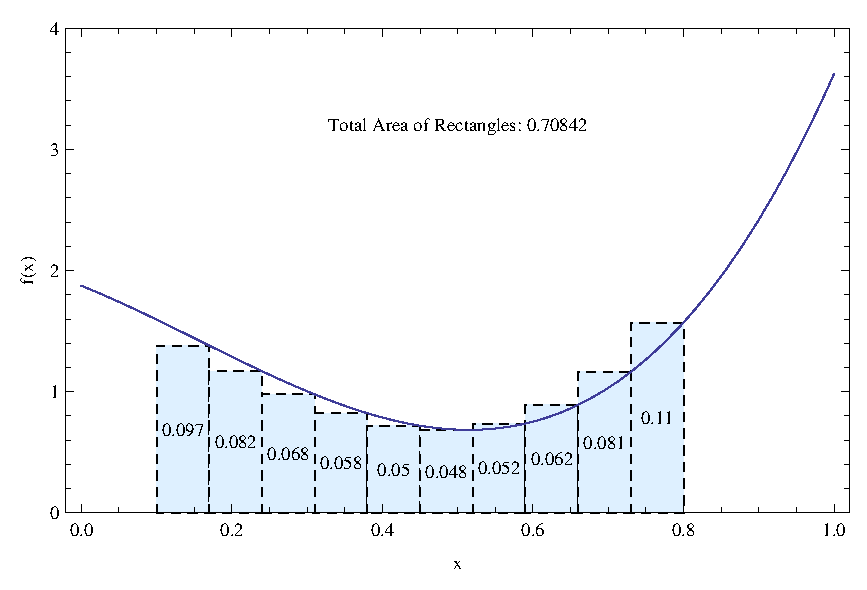
\includegraphics[scale=.6]{fig/rightrectangle-10.eps}}
  \caption{Numerical integration of $f(x) = (2 x-0.5)^3+(1.5 x-1)^2-x+1$ for $x$ in $[0.1,0.8]$
    by the (right) rectangle method for increasing values of $N$. The number inside each rectangle is
    the area of that rectangle, and the total area is displayed on each graph.
  The exact value of the integral is 0.70525.}\label{fig:rectangle}
\end{figure}

\section{Left Rectangle Method}\index{left rectangle method}\index{rectangle method!left}
\begin{seamlessnote}
  Now that we've described the rectangle method fairly well, including the math for
  each of the different versions, we will begin developing the code 
  for the left rectangle method.  The first step is to develop the tests, and
  every test needs an expected value against which to compare. The obvious way to test the code
  is to compare results against analytical values. 
  For the tests specified in \ref{req@4.1}-\ref{req@4.4}, we have analytic values. Also, since
  the functions are increasing or decreasing over the intervals specified, we can use an expression
  for the maximum error of the rectangle integration method in our tests.
\end{seamlessnote}

If $f(x)$ is increasing or decreasing on the interval $[a,b]$, the \textit{maximum error}, $E$, 
for left or right rectangle method numerical integration
\index{maximum error!left or right rectangle method}\index{left or right rectangle method maximum error}
  is given by
\begin{equation}
  E \leq \frac{b-a}{N}\left|f(b)-f(a)\right| \label{eq:lr-rectangle-max-error}
\end{equation}

We can create a helper function to compute the maximum error for left and right rectangle
methods using Equation~\ref{eq:lr-rectangle-max-error}. The calculated value will be used
in tests for the left and right rectangle methods to check that the result is within 
the maximum error expected for a given $a$, $b$, and $N$. 
\begin{enumspec}
\item\spec{1} Helper function \chpl{leftRightRectangleMaxErr}: compute the maximum error 
  expected for left or right rectangle method of numerical integration. \\
  \begin{tabular}{r r p{10cm}} \toprule
    \textbf{arguments} & \chpl{a:real} & lower bound \\ 
                       & \chpl{b:real} & upper bound \\ 
                       & \chpl{N:int}  & number of subintervals \\ 
                       & \chpl{f}      & function \\ \midrule
    \textbf{return}    & \chpl{:real}  & maximum error expected 
      for left or right rectangle method of numerical integration
      per Equation~\ref{eq:lr-rectangle-max-error} \\ \bottomrule
  \end{tabular}
\end{enumspec}

\begin{chapelhelper}{leftRightRectangleMaxErr.chpl}
  \begin{chapel}
proc leftRightRectangleMaxErr(a: real, b: real, N: int, f): real{
  return ((b-a)/N)*abs(f(b)-f(a));
}
  \end{chapel}
\end{chapelhelper}

\begin{seamlessnote}
  Our first specification, \ref{spec@1}, was created with the following \latex:\\
  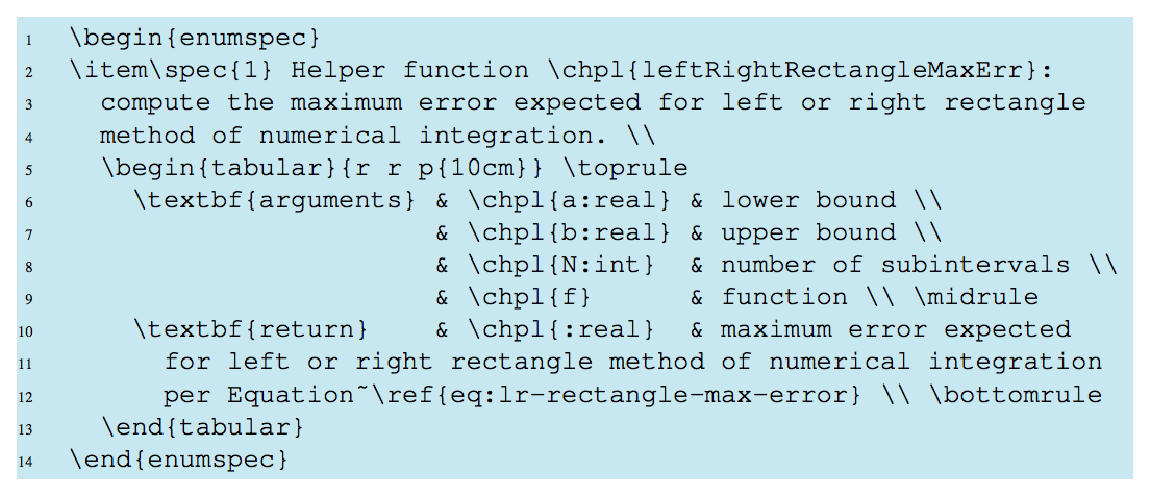
\includegraphics[scale=.6]{fig/s1_listing.eps}\\
Each specification is essentially an \verb|item| (see line 2) in an \verb|enumspec| environment, 
(see lines~1 and 14) which 
is defined in the file \path|seamless.sty| and is an extension of the \verb|enumerate| 
  environment.  These \verb|item|'s are labeled using the \verb|\spec{x}| command, where
  \verb|x| is the desired number in the label (\eg \verb|\spec{27}| to get \textbf{S27}).
  The convention in \seamless is that the specifications are numbered 
  consecutively, and they are referenced with the command \verb|\ref{spec@x}|.
  The appropriate format in which to present the code specification is the developer's
  choice. As seen in lines 5 through 13 above, the format used in this tutorial is to use
  the \verb|tabular| environment, with an ``argument'' group and a ``return'' group. As will
  be seen below, when a specification meets a requirement, another row is added to 
  annotate this.

  The helper files are chunks of code that are used to support
  testing that the developer wants to have outside of the tests. The most likely 
  reason being that
  the code contains setup or auxiliary functions that are used for multiple tests. In 
  our example
  above, we are using some foresight and envisioning that the \chpl{leftRightRectangleMaxErr}
  function will also be used in a test for the left rectangle numerical integration function. 
  To extract the helper files from the \latex source files, run the following command in the 
  directory containing the source:
\begin{verbatim}
[./tutorial/] $ make helpers
\end{verbatim}
  This command runs the \texttt{helpers} target in the Makefile at the root of the 
  tutorial directory (\path{./tutorial/Makefile}). A Makefile is a text 
  file written in a certain prescribed syntax. Together with the \texttt{make} utility, it 
  helps automate repetitive command-line tasks such as building software from its source files. 
  In this case, the \texttt{helpers} target cleans out the \path{./tutorial/helper} directory and
  executes the \path{./util/extract\_helpers} python script with the appropriate arguments.
\end{seamlessnote}

One of the functions that we need to test our methods against is $f(x) = x^3$, 
with $a=0$, $b=1$, and $N=100$.
Since the function is increasing on the interval $[0,1]$, we can use 
the helper function that we just created to compute the maximum expected error. We are
ready to create our first test for a function that we will write to compute the definite
integral using the left rectangle method. This function will be called 
\chpl{leftRectangleIntegration}
and will be written to \path{leftRectangleIntegration.chpl}.

  \begin{enumspec}
  \item\spec{2} Test \chpl{leftRectangleIntegrationTest1}: 
    integrates the function $x^3$ over the interval
    $[0,1]$ by the
    left rectangle numerical integration method with 100 subintervals and verifies
    that the result is within the expected maximum error of the exact value, 0.25.\\
    \begin{tabular}{r r p{6cm}} \toprule
      \textbf{output}      & \chpl{stdout: true}   & test passed \\ 
                           & \chpl{stdout: false}  & test failed \\ \midrule
      \textbf{modules loaded}     & \multicolumn{2}{l}{\chpl{leftRightRectangleMaxErr}} \\
                                  & \multicolumn{2}{l}{\chpl{leftRectangleIntegration}} \\ \midrule
      \textbf{requirements met} & \multicolumn{2}{l}{\meetsreq{4.1}} \\ \midrule
  \end{tabular}
  \end{enumspec}

  \begin{seamlessnote}
    The first test specification, \ref{spec@2}, differs quite a bit from \ref{spec@1}, which was
    for a helper function. This first test is an executable to be compiled and run without any 
    input, and the output is written to \chpl{stdout}, Therefore, we have a row for the 
    potential outputs, but not input, arguments, or a return value. We also load two modules
    in this test, so there is a row to annotate those.  Finally, this test meets one of the
    requirements, \ref{req@4.1}, and that fact is annotated in the ``requirements met'' row.
    To annotate this, we use the command \verb|\meetsreq{x}|, where \verb|x| is the number of the
    requirement that is met (\eg \verb|\meetsreq{4.1}| to annotate that Requirement~\textbf{R4.1}
    is met).
  \end{seamlessnote}

  \begin{chapeltest}{leftRectangleIntegrationTest1.chpl}
    A test for function \chpl{leftRectangleIntegration} using $f(x) = x^3$.
    \begin{chapelpre}
    \end{chapelpre}
    \begin{chapel}
use leftRightRectangleMaxErr;
use leftRectangleIntegration;

proc f(x:real):real {
  return x**3;
} 

var calculated:real;
var exact:real = 0.25;
var maximumError:real = leftRightRectangleMaxErr(
  a = 0.0, b = 1.0, N = 100, f = f);
var verified:bool;

calculated = leftRectangleIntegration(
  a = 0.0, b = 1.0, N = 100, f = f);
verified = (abs(calculated - exact) <= maximumError);
writeln(verified);
    \end{chapel}
    \begin{chapelpost}
    \end{chapelpost}
    \begin{chapeloutput}
true
    \end{chapeloutput}
  \end{chapeltest}

  \begin{seamlessnote}
    The above test is inserted with the following \latex code: \\
    \includegraphics[scale=.6]{fig/s2_listing.eps}\\
    Tests are inserted within \verb|chapeltest| environments (see lines~1 and~29). The option
    passed to the environment is the filename for the test. Each test is given a unique filename.
    The text following the \verb|\begin{chapeltest}| command is printed in the PDF, but is 
      discarded when the test is extracted from the \latex source.  Inside the \verb|chapeltest|
      environment, four other environments are declared: 
      \begin{itemize}
        \item \verb|chapelpre|: code inserted at beginning of the test but not printed in the PDF
        \item \verb|chapel|: test code
        \item \verb|chapelpost|: code inserted at end of test but not printed in the PDF
        \item \verb|chapeloutput|: \chpl{stdout} output for a passed test; text is extracted to a file
          with the same base filename as the test with a \path{.good} extension
      \end{itemize}

    Now that we have our first test written, we need to extract it from the latex source and verify
    that it does not pass.
    To extract the test from the latex source and run it:
    \begin{verbatim}
[./tutorial/] $ make tests
[./tutorial/] $ make test
    \end{verbatim}
    These commands run the \verb|tests| and \verb|test| targets in the same Makefile referenced above.
    In this case, the \verb|tests| target cleans out the \path{./tutorial/test} directory and
    executes the \path{./util/extract_tests} python script with the appropriate arguments.
    The \verb|test| target changes to the \path{./tutorial/test} directory and 
    executes the \verb|start_test| script that comes with
    the chapel distribution (in the \path{CHPL_HOME/util} directory). The script compiles 
      and executes each of the
    chapel source files in the test directory 
    (\eg \path{leftRectangleIntegrationTest1.chpl} as in the example above) 
    and compares the output with the contents of a file with a \path{.good} extension
    (\eg \path{leftRectangleIntegrationTest1.good} for the above test). 
    The last few lines of output should look something like this:
    \begin{verbatim}
[Test Summary - 150107.202408]
[Summary: #Successes = 0 | #Failures = 1 | #Futures = 0 | #Warnings = 0 ]
[END]
    \end{verbatim}
  \end{seamlessnote}

  \begin{TODO}
    Update test target to run all targets necessary to run tests.
  \end{TODO}
  \begin{TODO}
    Refactor \verb|chapeltest| environment to \verb|test|.  (Similarly for 
      \verb|chapelsource| and \verb|chapelhelper| environments.)
  \end{TODO}
  \begin{TODO}
    Add option to gobble spaces on left side in \verb|chapeltest| so that code can be
    indented in source.
  \end{TODO}

  The code that provides the \chpl{leftRectangleIntegration} function is straightforward.
  \begin{enumspec}
  \item\spec{3} Function \chpl{leftRectangleIntegration}: 
    integrates a function by the left rectangle method of numerical integration.\\
  \begin{tabular}{r r p{10cm}} \toprule
    \textbf{arguments} & \chpl{a:real} & lower bound \\ 
                       & \chpl{b:real} & upper bound \\ 
                       & \chpl{N:int}  & number of subintervals \\ 
                       & \chpl{f}      & function \\ \midrule
    \textbf{return}    & \chpl{:real}  & definite integral 
      computed by left rectangle method of numerical integration
      per Equations~\ref{eq:rectangle} and \ref{eq:subinterval-width} 
      and the appropriate expression for $x_n$ in Table~\ref{tab:xn-rectangle}\\ \bottomrule
    \textbf{requirements met} & \multicolumn{2}{l}{\meetsreq{1.1,2,3}} \\ \midrule
  \end{tabular}
  \end{enumspec}

  \begin{chapelsource}{leftRectangleIntegration.chpl}
    \begin{chapel}
proc leftRectangleIntegration(a: real, b: real, N: int, f): real{
  var h: real = (b - a)/N; 
  var sum: real = 0.0;
  var x_n: real;
  for n in 0..N-1 {
    x_n = a + n * h;
    sum = sum + f(x_n);
  }
  return h * sum;
}
    \end{chapel}
  \end{chapelsource}

  \begin{seamlessnote}
    Our first chunk of source code is inserted with the following \latex source:\\
    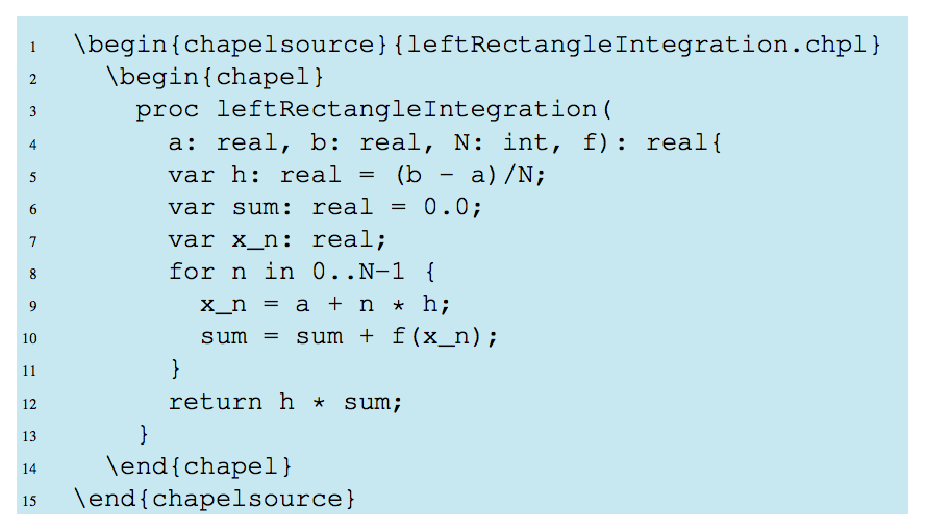
\includegraphics[scale=.6]{fig/s3_listing.eps}\\
    The source is specified in a \verb|chapel| environment (see lines~2 and~14) within 
    a \verb|chapelsource| environment (see lines~1 and~15). The option passed to the
    \verb|\begin{chapelsource}| command specifies the file in which the source is placed.
    Multiple chunks of source can be extracted into a given source file.

    We can now verify that test \path{leftRectangleIntegrationTest1} passes. First
    we need to extract the chapel source from our \latex file and then run the test that was
    written previously:
  \begin{verbatim}
[./tutorial/] $ make sources
[./tutorial/] $ make test
  \end{verbatim}
  These commands run the \verb|sources| and \verb|test| targets in the Makefile.
  In this case, the \verb|sources| target cleans out the \path{./tutorial/source} directory and
  executes the \path{./util/extract_sources} python script with the appropriate arguments, putting
  the source code that we've defined in our latex file into the \path{./tutorial/source} directory.
  The last few lines of output should now look something like this:
  \begin{verbatim}
[Test Summary - 150107.202408]
[Summary: #Successes = 1 | #Failures = 0 | #Futures = 0 | #Warnings = 0 ]
[END]
  \end{verbatim}
\end{seamlessnote}

Another of the functions that we need to test our methods against is 
$f(x) = 1/x$, where $x$ is $[1,100]$, with 1,000 approximations. 
The exact result is the natural log of 100, or about 4.605170.
Since the function is decreasing on the interval $[1,100]$, we can again use 
the helper function in \lstinline{leftRightRectangleMaxErr.chpl} to compute the 
maximum expected error.  
Our second test 
for the left rectangle method is very similar to the first. 
\begin{enumspec}
\item\spec{4} Test \chpl{leftRectangleIntegrationTest2.chpl}: 
    integrates the function $1/x$ over the interval
    $[1,100]$ by the
    left rectangle numerical integration method with 1000 subintervals and verifies
    that the result is within the expected maximum error of the exact value, $ln(100)$.\\
    \begin{tabular}{r r p{6cm}} \toprule
      \textbf{output}      & \chpl{stdout: true}   & test passed \\ 
                           & \chpl{stdout: false}  & test failed \\ \midrule
      \textbf{modules loaded}     & \multicolumn{2}{l}{\chpl{leftRightRectangleMaxErr}} \\
                                  & \multicolumn{2}{l}{\chpl{leftRectangleIntegration}} \\ \midrule
      \textbf{requirements met} & \multicolumn{2}{l}{\meetsreq{4.2}} \\ \midrule
  \end{tabular}
\end{enumspec}

\begin{chapeltest}{leftRectangleIntegrationTest2.chpl}
  A test for function \chpl{leftRectangleIntegration} using $f(x) = 1/x$.
  \begin{chapelpre}
  \end{chapelpre}
  \begin{chapel}
use leftRightRectangleMaxErr;
use leftRectangleIntegration;

proc f(x:real):real {
  return 1/x;
} 

var exact:real = 4.605170; 
var maximumError:real = 
  leftRightRectangleMaxErr(a = 1.0, b = 100.0, N = 1000, f = f);
var calculated: real = 
  leftRectangleIntegration(a = 1.0, b = 100.0, N = 1000, f = f);
var verified: bool = (abs(calculated - exact) <= maximumError);
writeln(verified);
  \end{chapel}
  \begin{chapelpost}
  \end{chapelpost}
  \begin{chapeloutput}
true
  \end{chapeloutput}
\end{chapeltest}

\begin{seamlessnote}
  By now you have likely realized that we already have some opportunities to refactor code in
  our first two tests above. The tests are very similar except for the expressions in the 
  test function ($f$), the exact values for the integrals, and the values of $a$, $b$, and $N$
  passed to \chpl{leftRightRectangleMaxErr} and \chpl{leftRectangleIntegration}.
  Also, you'll notice that the arguments to 
  \chpl{leftRightRectangleMaxErr} and \chpl{leftRectangleIntegration}
  are identical, and perhaps it would be good to always get the maximum error associated with a
  numerical integration.
  We will rewrite our integration function to return the value of the integral and
  the maximum error in a tuple. 
  We can also combine the two tests and add the final two tests for the function $f(x) = x$.
  Thinking ahead a little, we can put the test functions into a helper module since they will
  be the same for every test.
  In practice, the developer would typically not keep the above two tests. She would 
  replace the above two tests with what follows and the resulting \lstinline{seamless} 
  document would be much more streamlined than what is presented here. Of course, there is no 
  harm in keeping all of the versions of the tests.
\end{seamlessnote}

\begin{TODO}
  Add description of versioning with git.
\end{TODO}

\begin{enumspec}
\item\spec{5} Helper \chpl{testFunctions.chpl}: 
  provide the functions $f(x) \in \{x^3, 1/x, x\}$ for use in tests. \\
  \begin{tabular}{r r l} \toprule
    \textbf{proc f1} & & \\ \midrule
    \textbf{arguments} & \chpl{x:real} & $x$ \\ \midrule
    \textbf{return}    & \chpl{:real}  & $x^3$ \\ \bottomrule
    \textbf{proc f2} & & \\ \midrule
    \textbf{arguments} & \chpl{x:real} & $x$ \\ \midrule
    \textbf{return}    & \chpl{:real}  & $1/x$ \\ \bottomrule
    \textbf{proc f3} & & \\ \midrule
    \textbf{arguments} & \chpl{x:real} & $x$ \\ \midrule
    \textbf{return}    & \chpl{:real}  & $x$ \\ \bottomrule
  \end{tabular}
\end{enumspec}

\begin{chapelhelper}{testFunctions.chpl}
  \begin{chapel}
proc f1(x:real):real {
  return x**3;
} 
proc f2(x:real):real {
  return 1/x;
} 
proc f3(x:real):real {
  return x;
} 
  \end{chapel}
\end{chapelhelper}

  \begin{enumspec}
  \item\spec{6} Test \chpl{leftRectangleIntegrationTest3}: 
    integrates test functions according to Requirements~\ref{req@4.1} through~\ref{req@4.4}.\\
    \begin{tabular}{r r p{6cm}} \toprule
      \textbf{output} x 4  & \chpl{stdout: true}   & test passed \\ 
                           & \chpl{stdout: false}  & test failed \\ \midrule
      \textbf{modules loaded} & \multicolumn{2}{l}{\chpl{testFunctions}} \\
                              & \multicolumn{2}{l}{\chpl{leftRectangleIntegrationWithErr}} \\ \midrule
      \textbf{requirements met} & \multicolumn{2}{l}{\meetsreq{4.1,4.2,4.3,4.4}} \\ \bottomrule
  \end{tabular}
  \end{enumspec}

\begin{chapeltest}{leftRectangleIntegrationTest3.chpl}
  A test for \chpl{leftRectangleIntegrationWithErr} using $f(x) \in \{x^3, 1/x, x\}$.
  \begin{chapelpre}
  \end{chapelpre}
  \begin{chapel}
use leftRectangleIntegrationWithErr;
use testFunctions;

var exact:real;
var calculated:real;
var maxErr:real;

exact = 0.25;
(maxErr, calculated) = leftRectangleIntegrationWithErr(
  a = 0.0, b = 1.0, N = 100, f = f1);
writeln((abs(calculated - exact) <= maxErr));

exact = 4.605170;
(maxErr, calculated) = leftRectangleIntegrationWithErr(
  a = 1.0, b = 100.0, N = 1000, f = f2);
writeln((abs(calculated - exact) <= maxErr));

exact = 12500000;
(maxErr, calculated) = leftRectangleIntegrationWithErr(
  a = 0.0, b = 5000.0, N = 5000000, f = f3);
writeln((abs(calculated - exact) <= maxErr));

exact = 18000000;
(maxErr, calculated) = leftRectangleIntegrationWithErr(
  a = 0.0, b = 6000.0, N = 6000000, f = f3);
writeln((abs(calculated - exact) <= maxErr));
  \end{chapel}
  \begin{chapelpost}
  \end{chapelpost}
  \begin{chapeloutput}
true
true
true
true
  \end{chapeloutput}
\end{chapeltest}

\begin{enumspec}
\item\spec{7} Function \chpl{leftRectangleIntegrationWithErr}: 
  computes the definite integral of a function by the left rectangle
    method of numerical integration. Also computes the maximum expected error.\\
  \begin{tabular}{r r p{10cm}} \toprule
    \textbf{arguments} & \chpl{a:real} & lower bound \\ 
                       & \chpl{b:real} & upper bound \\ 
                       & \chpl{N:int}  & number of subintervals \\ 
                       & \chpl{f}      & function \\ \midrule
    \textbf{return}    & \chpl{:real}  & definite integral 
      computed by left rectangle method of numerical integration
      per Equations~\ref{eq:rectangle} and \ref{eq:subinterval-width} 
      and the appropriate expression for $x_n$ in Table~\ref{tab:xn-rectangle}
      is first element of two-element tuple\\ 
                       & \chpl{:real}  & maximum error expected 
      per Equation~\ref{eq:lr-rectangle-max-error} is second element of two-element
      tuple \\ \midrule
    \textbf{requirements met} & \multicolumn{2}{l}{\meetsreq{1.1,2,3}} \\ \bottomrule
  \end{tabular}
\end{enumspec}

\begin{chapelsource}{leftRectangleIntegrationWithErr.chpl}
  \begin{chapel}
proc leftRectangleIntegrationWithErr(
  a: real, b: real, N: int, f): 2*real{
  var maxErr: real = ((b-a)/N)*abs(f(b)-f(a));
  var h: real = (b - a)/N; 
  var sum: real = 0.0;
  var x_n: real;
  for n in 0..N-1 {
    x_n = a + n * h;
    sum = sum + f(x_n);
  }
  return (h * sum, maxErr);
}
  \end{chapel}
\end{chapelsource}

\section{Right Rectangle Method}

  \begin{enumspec}
  \item\spec{8} Test \chpl{rightRectangleIntegrationTest}: 
    integrates test functions according to Requirements~\ref{req@4.1} through~\ref{req@4.4}
    using the right rectangle numerical integration method and compares results
    to expected maximum error.\\
    \begin{tabular}{r r p{6cm}} \toprule
      \textbf{output} x 4  & \chpl{stdout: true}   & test passed \\ 
                           & \chpl{stdout: false}  & test failed \\ \midrule
      \textbf{modules loaded} & \multicolumn{2}{l}{\chpl{testFunctions}} \\
                              & \multicolumn{2}{l}{\chpl{rightRectangleIntegrationWithErr}} \\ \midrule
      \textbf{requirements met} & \multicolumn{2}{l}{\meetsreq{4.1,4.2,4.3,4.4}} \\ \bottomrule
  \end{tabular}
  \end{enumspec}

\begin{chapeltest}{rightRectangleIntegrationTest.chpl}
  A test for \lstinline{rightRectangleIntegrationWithErr} using $f(x) \in \{x^3, 1/x, x\}$.
  \begin{chapelpre}
  \end{chapelpre}
  \begin{chapel}
use rightRectangleIntegrationWithErr;
use testFunctions;

var exact:real;
var calculated:real;
var maxErr:real;

exact = 0.25;
(maxErr, calculated) = rightRectangleIntegrationWithErr(
  a = 0.0, b = 1.0, N = 100, f = f1);
writeln((abs(calculated - exact) <= maxErr));

exact = 4.605170;
(maxErr, calculated) = rightRectangleIntegrationWithErr(
  a = 1.0, b = 100.0, N = 1000, f = f2);
writeln((abs(calculated - exact) <= maxErr));

exact = 12500000;
(maxErr, calculated) = rightRectangleIntegrationWithErr(
  a = 0.0, b = 5000.0, N = 5000000, f = f3);
writeln((abs(calculated - exact) <= maxErr));

exact = 18000000;
(maxErr, calculated) = rightRectangleIntegrationWithErr(
  a = 0.0, b = 6000.0, N = 6000000, f = f3);
writeln((abs(calculated - exact) <= maxErr));
  \end{chapel}
  \begin{chapelpost}
  \end{chapelpost}
  \begin{chapeloutput}
true
true
true
true
  \end{chapeloutput}
\end{chapeltest}

\begin{enumspec}
\item\spec{9} Function \chpl{rightRectangleIntegrationWithErr}: 
  computes the definite integral of a function by the right rectangle
    method of numerical integration. Also computes the maximum expected error.\\
  \begin{tabular}{r r p{10cm}} \toprule
    \textbf{arguments} & \chpl{a:real} & lower bound \\ 
                       & \chpl{b:real} & upper bound \\ 
                       & \chpl{N:int}  & number of subintervals \\ 
                       & \chpl{f}      & function \\ \midrule
    \textbf{return}    & \chpl{:real}  & definite integral 
      computed by right rectangle method of numerical integration
      per Equations~\ref{eq:rectangle} and \ref{eq:subinterval-width} 
      and the appropriate expression for $x_n$ in Table~\ref{tab:xn-rectangle}
      is first element of two-element tuple\\ 
                       & \chpl{:real}  & maximum error expected 
      per Equation~\ref{eq:lr-rectangle-max-error} is second element of two-element
      tuple \\ \midrule
    \textbf{requirements met} & \multicolumn{2}{l}{\meetsreq{1.2,2,3}} \\ \bottomrule
  \end{tabular}
\end{enumspec}

\begin{chapelsource}{rightRectangleIntegrationWithErr.chpl}
  \begin{chapel}
proc rightRectangleIntegrationWithErr(
  a: real, b: real, N: int, f): 2*real{
  var maxErr: real = ((b-a)/N)*abs(f(b)-f(a));
  var h: real = (b - a)/N; 
  var sum: real = 0.0;
  var x_n: real;
  for n in 0..N-1 {
    x_n = a + (n + 1) * h;
    sum = sum + f(x_n);
  }
  return (h * sum, maxErr);
}
  \end{chapel}
\end{chapelsource}

\section{Midpoint Rectangle Method}\label{sec:midpoint-rectangle-method}
For a function $f$ which is twice differentiable, the maximum error $E$ for the
midpoint rectangle method is given by the following equation:
\begin{equation}
  E \leq \frac{(b-a)^3}{24 N^2} f''(\xi) \label{eq:mp-rectangle-max-error}
\end{equation}
for some $\xi$ in $[a,b]$.

Unlike the left and right rectangle methods, it is more difficult to write a function
to determine the maximum expected error for the midpoint version. First, we must 
determine the maximum value of
the second derivative before we can compute the maximum error using 
Equation~\ref{eq:mp-rectangle-max-error}. 
For $f(x) = x^3$, the second derivative is $f''(x) = 6x$. On the interval specified by
Requirement~\ref{req@4.1}, $[0,1]$, the maximum value is $f''(1) = 6$.
For $f(x) = 1/x$, the second derivative is $f''(x) = 2x^{-3}$. On the interval specified by
Requirement~\ref{req@4.2}, $[1,100]$, the maximum value is $f''(1) = 2$.
The function $f(x) = x$ specified by Requirement~\ref{req@4.3} and \ref{req@4.4}, does not have
a second derivative. The midpoint method is expected to give a very accurate answer for this function,
so we will use a value of 0.00001 for the maximum expected error for the two final tests.
The calculated maximum expected error for the tests specified in Requirements~\ref{req@4.1} and
\ref{req@4.2} are given in Table~\ref{tab:midpoint-rectangle-error}.

\begin{table}[htbp]
  \centering
  \caption{Values for expressions in Equation~\ref{eq:mp-rectangle-max-error} and the maximum 
    expected error of the midpoint rectangle method of numerical integration for 
    $f(x) \in \{x^3, 1/x\}$.}
  \label{tab:midpoint-rectangle-error}
  \begin{tabular}{ccccc}
    \textbf{Function} & \textbf{Interval} & \textbf{N} & \textbf{Maximum $f''(x)$} & $E$  \\ \toprule
    $x^3$ & $[0,1]$   & 100  & 6 & 0.000025 \\ \midrule
    $1/x$ & $[1,100]$ & 1000 & 3 & 0.121287 \\ \bottomrule
  \end{tabular}
\end{table}

  \begin{enumspec}
  \item\spec{10} Test \chpl{midpointRectangleIntegrationTest}: 
    integrates test functions according to Requirements~\ref{req@4.1} through~\ref{req@4.4}
    using the midpoint rectangle numerical integration method and compares results
    to the maximum expected error.\\
    \begin{tabular}{r r p{6cm}} \toprule
      \textbf{output} x 4  & \chpl{stdout: true}   & test passed \\ 
                           & \chpl{stdout: false}  & test failed \\ \midrule
      \textbf{modules loaded} & \multicolumn{2}{l}{\chpl{testFunctions}} \\
                              & \multicolumn{2}{l}{\chpl{midpointRectangleIntegration}} \\ \midrule
      \textbf{requirements met} & \multicolumn{2}{l}{\meetsreq{4.1,4.2,4.3,4.4}} \\ \bottomrule
  \end{tabular}
  \end{enumspec}

\begin{chapeltest}{midpointRectangleIntegrationTest.chpl}
  A test for \lstinline{midpointRectangleIntegration} using $f(x) \in \{x^3, 1/x, x\}$.
  \begin{chapelpre}
  \end{chapelpre}
  \begin{chapel}
use midpointRectangleIntegration;
use testFunctions;

var exact:real;
var calculated:real;
var maxErr:real;

exact = 0.25;
maxErr = 0.000025;
calculated = midpointRectangleIntegration(
  a = 0.0, b = 1.0, N = 100, f = f1);
writeln((abs(calculated - exact) <= maxErr));

exact = 4.605170;
maxErr = 0.121287;
calculated = midpointRectangleIntegration(
  a = 1.0, b = 100.0, N = 1000, f = f2);
writeln((abs(calculated - exact) <= maxErr));

exact = 12500000;
maxErr = 0.00001;
calculated = midpointRectangleIntegration(
  a = 0.0, b = 5000.0, N = 5000000, f = f3);
writeln((abs(calculated - exact) <= maxErr));

exact = 18000000;
maxErr = 0.00001;
calculated = midpointRectangleIntegration(
  a = 0.0, b = 6000.0, N = 6000000, f = f3);
writeln((abs(calculated - exact) <= maxErr));
  \end{chapel}
  \begin{chapelpost}
  \end{chapelpost}
  \begin{chapeloutput}
true
true
true
true
  \end{chapeloutput}
\end{chapeltest}

\begin{enumspec}
\item\spec{11} Function \chpl{midpointRectangleIntegration}: 
  computes the definite integral of a function by the midpoint rectangle
  method of numerical integration.\\
  \begin{tabular}{r r p{10cm}} \toprule
    \textbf{arguments} & \chpl{a:real} & lower bound \\ 
                       & \chpl{b:real} & upper bound \\ 
                       & \chpl{N:int}  & number of subintervals \\ 
                       & \chpl{f}      & function \\ \midrule
    \textbf{return}    & \chpl{:real}  & definite integral 
      computed by midpoint rectangle method of numerical integration
      per Equations~\ref{eq:rectangle} and \ref{eq:subinterval-width} 
      and the appropriate expression for $x_n$ in Table~\ref{tab:xn-rectangle}\\
    \textbf{requirements met} & \multicolumn{2}{l}{\meetsreq{1.3,2,3}} \\ \bottomrule
  \end{tabular}
\end{enumspec}

\begin{chapelsource}{midpointRectangleIntegration.chpl}
  \begin{chapel}
proc midpointRectangleIntegration(
  a: real, b: real, N: int, f): real{
  var h: real = (b - a)/N; 
  var sum: real = 0.0;
  var x_n: real;
  for n in 0..N-1 {
    x_n = a + (n + 0.5) * h;
    sum = sum + f(x_n);
  }
  return h * sum;
}
  \end{chapel}
\end{chapelsource}
